
%(BEGIN_QUESTION)
% Copyright 2008, Tony R. Kuphaldt, released under the Creative Commons Attribution License (v 1.0)
% This means you may do almost anything with this work of mine, so long as you give me proper credit

Identify the state of the light bulb when the normally-open pressure switch contact {\it closes}:

$$\includegraphics[width=15.5cm]{i03203x01.eps}$$

Assuming the light bulb functions as a pressure alarm to alert operators to an unsafe condition, determine whether this is a {\it low-pressure} alarm or a {\it high pressure} alarm.

\vfil 

Hint: remember that the ``normal'' status of a switch is defined as the status of {\it minimum stimulus}: when the switch is exposed to the lowest possible degree of process stimulation (in this particular case, to the lowest possible pressure).

\underbar{file i03203}
\eject
%(END_QUESTION)





%(BEGIN_ANSWER)

This is a graded question -- no answers or hints given!
 
%(END_ANSWER)





%(BEGIN_NOTES)

When the pressure switch contact closes, the relay energizes, opening the normally-closed relay contact and turning the light off.

\vskip 10pt

This circuit functions as a {\it low-pressure} alarm, turning the light bulb on if the process pressure ever drops below the switch's trip value.

%INDEX% Pictorial circuit review (relay circuit)

%(END_NOTES)


